\documentclass[a4paper, 12pt]{article}

\usepackage{hyperref}
\usepackage[warn]{mathtext}
\usepackage[utf8]{inputenc}
\usepackage[T2A]{fontenc}
\usepackage[english,russian]{babel}
\usepackage{multirow}
\usepackage{float}
\restylefloat{table}
\usepackage{amsmath,amsfonts,amssymb,amsthm,mathtools}
\usepackage{indentfirst}
\DeclareSymbolFont{T2Aletters}{T2A}{cmr}{m}{it}
\usepackage{ gensymb }
\mathtoolsset{showonlyrefs=true}
\usepackage{euscript}
\usepackage{mathrsfs}
\usepackage[left=2cm,right=2cm,top=2cm,bottom=2cm]{geometry}
\usepackage{graphicx}
\usepackage{wrapfig}
\usepackage[rgb]{xcolor}
\hypersetup{
colorlinks=true,
urlcolor=blue
}
\usepackage{tikz}

\title{Лабораторная работа}
\author{Гисич Арсений Б03-102}
\date{2023}

\begin{document}

	\begin{center}
		{\large МОСКОВСКИЙ ФИЗИКО-ТЕХНИЧЕСКИЙ ИНСТИТУТ (НАЦИОНАЛЬНЫЙ ИССЛЕДОВАТЕЛЬСКИЙ УНИВЕРСИТЕТ)}
	\end{center}
	\vspace{5 cm}
	{\Large
		\begin{center}
			{\bf Лабораторная работа 4.3.1}\\[0.2 cm]
			Дифракция света
		\end{center}
	}
	\vspace{4 cm}
	\begin{flushright}
		{\Large Выполнили: \\
			\vspace{0.2 cm}
			Гисич Арсений \\
            Айрапетян Микаел \\
			\vspace{0.2 cm}
			Б03-102 \\}
	\end{flushright}
	\vspace{8 cm}
	\begin{center}
		Долгопрудный\\[0.1 cm]
		2023
	\end{center}
\thispagestyle{empty}

\section{Аннотация}

В данной работе были исследованы явления дифракции Френеля и Фраунгофера на щели; было изучено влияние дифракции на разрешающую способность оптических инструментов.

\section{Теоретические сведения}

\subsection{Дифракция Френеля на щели}

Распределение интенсивности света в плоскости наблюдения (см. рис. \ref{fig:дифракцияФренеляУстановка}) проще всего рассчитывать с помощью зон Шустера. При освещении щели $ S_2 $ параллельным пучком лучей зоны Шустера представляют собой полоски, параллельные краям щели, изображённые на рис. \ref{fig:ШустерЗоны}. 

\begin{figure}[h!]
	\centering
	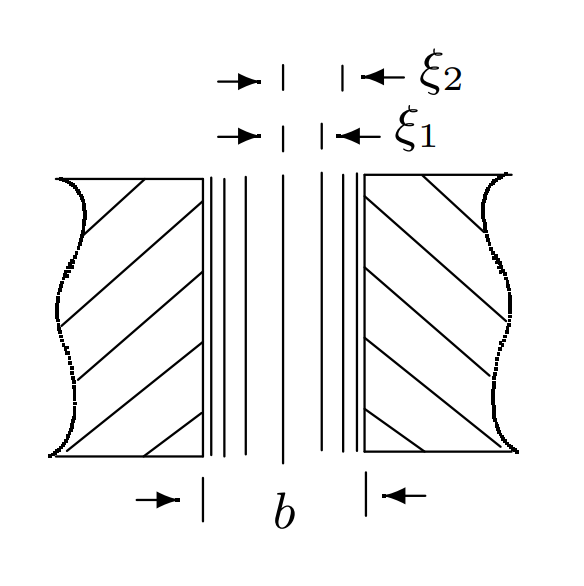
\includegraphics[width=0.5\linewidth]{1.png}
	\caption{Зоны Шустера, наблюдаемые при дифракции Френеля на щели}
	\label{fig:ШустерЗоны}
\end{figure}

Суммарная ширина $ n $ зон Шустера определяется соотношением:
\begin{equation}\label{eq:шустерзоны}
	\xi_n = \sqrt{n z \lambda},
\end{equation}
где $ \lambda $ -- длина волны; $ z $ -- расстояние между щелью и экраном.

Наблюдаемая на экране картина определяется волновым параметром:
\begin{equation}\label{eq:волновойПараметр}
	p = \frac{z \lambda}{b},
\end{equation}
где $ b $ -- толщина щели $ S_2 $. При $ p\ll 1 $ дифракция отсутствует (действует приближение геометрической оптики). При $ p\simeq 1 $ возникает дифракция Френеля с числом тёмных полос $ m $, тогда число зон на полуширине щели $ n = m+1 $.

Также можно ввести число Френеля, как число открытых зон на всей ширине щели:
\begin{equation}\label{eq:числоФренеля}
	C = \frac{b^2}{z \lambda} = \frac{1}{p^2}.
\end{equation}

\subsection{Дифракция Фраунгофера на щели}

При $ C\ll 1  $ наблюдается дифракция Фраунгофера с характерным распределением интенсивностей (см \ref{fig:Фраунгофер}). 

В центре поля зрения наблюдается дифракционный максимум. При малых углах $ \theta $ положение минимумов определяется соотношением:
\begin{equation*}\label{key}
	\theta_m = \frac{m \lambda}{b}.
\end{equation*}
Тогда расстояние от тёмной полосы до оптической оси $ O_2 $ равно:
\begin{equation}\label{eq:ФраунгоферМинимумы}
	x_m = m \frac{\lambda}{b} f_2,
\end{equation}
где $ f_2 $ -- фокус объектива.

\subsection{Дифракция Фраугофера на двух щелях}

Угловая координата $ \theta_m $ интерференционного максимума $ m $-го порядка определяется соотношением:
\begin{equation*}\label{key}
	\theta_m = \frac{m \lambda}{d},
\end{equation*}
где $ d $ -- расстояние между щелями. Тогда линейное расстояние между соседними интерференционными полосами равно:
\begin{equation}\label{eq:ИнтерфПолосыФраунгоф2}
	\delta x = \frac{\lambda}{d} f_2.
\end{equation}

Оценим число интерференционных полос в главном максимуме из соображений, что распределение интенсивностей такое же, как у одиночной щели (изображено пунктирной линией на рис. \ref{fig:Фраунгофер3}):
\begin{equation}\label{eq:числоЛиний}
	n = \frac{2 \lambda f_2}{b} \frac{1}{\delta x} = \frac{2 d}{b}.
\end{equation}

\begin{figure}[h!]
	\centering
	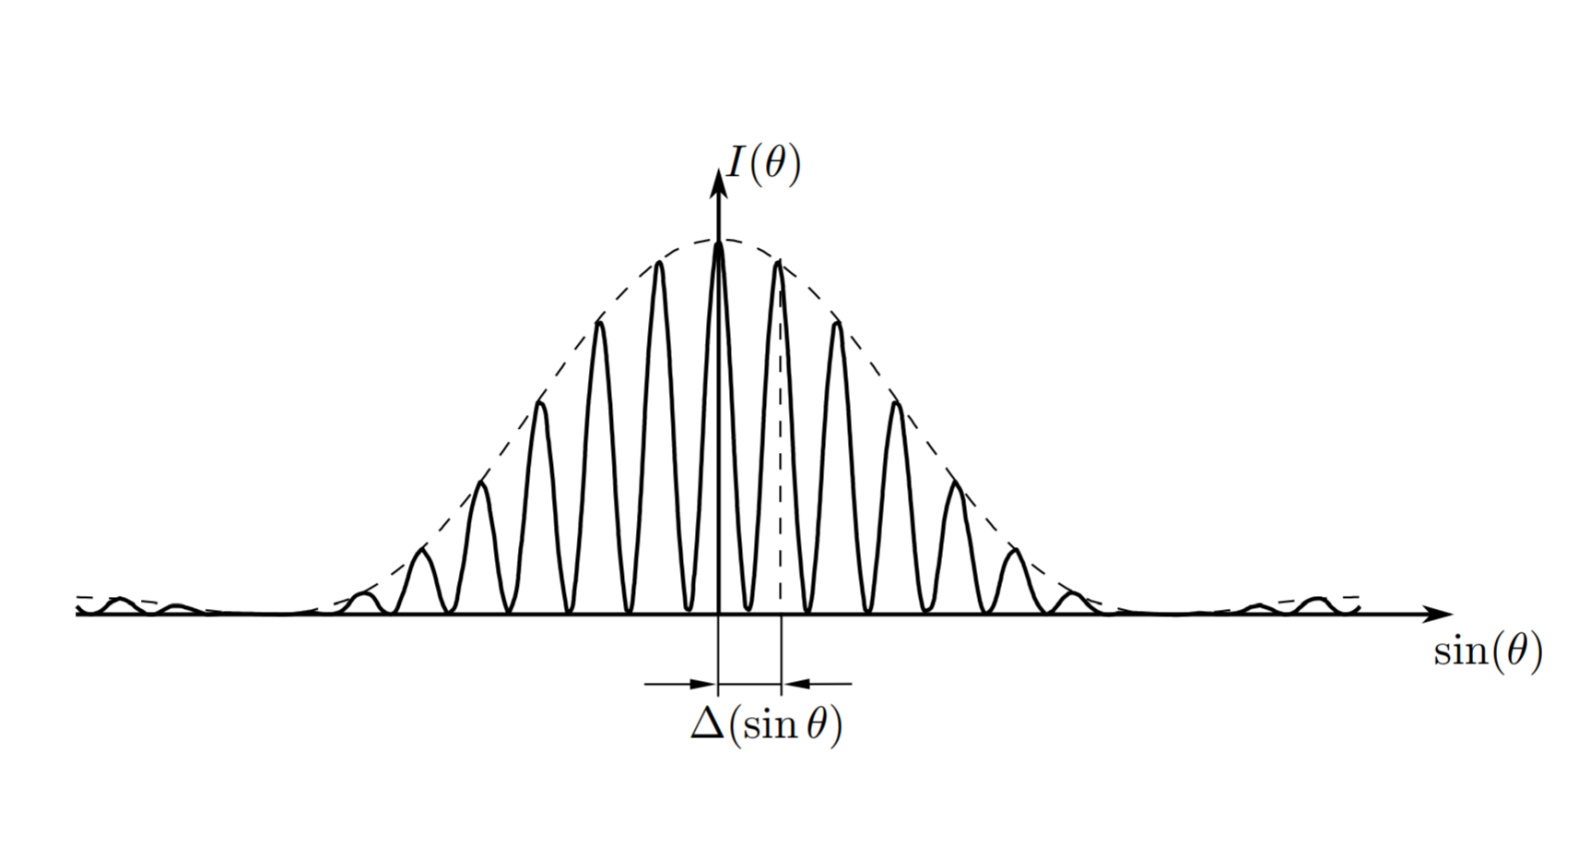
\includegraphics[width=0.8\linewidth]{5.png}
	\caption{Распределение интенсивностей в опыте с двумя щелями}
	\label{fig:Фраунгофер3}
\end{figure}


Для наблюдения интерференции требуется выполнение условия:
\begin{equation*}\label{eq:условиесрадиусом}
	d\le \rho_{ког} = \frac{\lambda}{b} f_1,
\end{equation*}
где $ \rho_{ког} $ -- радиус когерентности, $ b / f_1 $ -- угловая ширина входной щели $ S_1 $.

\subsection{Влияние дифракции на разрешающую способность оптического инструмента}

Установку на рис. \ref{fig:послустановка} можно рассматривать как оптический прибор. Для выявления его предельной разрешающей способности (ограниченной дифракцией на щели $ S_2 $) применяют критерий Рэлея:
\begin{equation}\label{eq:рэлей}
	\frac{\lambda}{D_0} = \frac{l}{f_2} = \frac{d}{f_1},
\end{equation}
где $ D_0 $ -- ширина щели $ S_0 $, $ l $ -- расстояние между изображениями щелей, $ d $ -- расстояние между щелями.

\section{Используемое оборудование}

\begin{enumerate}
    \item Микроскоп на поперечных салазках с микрометрическим винтом: \\ $ \Delta_{винта} = 1мкм; \Delta_{шкалы} = 0.02 мм $
    \item Светофильтр: $ \lambda = 5461\text{\AA}$
    \item Щели с регулируемой шириной: $ \Delta = 1 мкм $
    \item Оптическая скамья;
    \item Ртутная лампа; 
    \item Рамка с вертикальной нитью;
    \item Двойная щель;
    \item Зрительная труба
\end{enumerate}

Установки, применяемые в опыте, изображены на рис. \ref{fig:дифракцияФренеляУстановка}, \ref{fig:Фраунгофер}, \ref{fig:Фраунгофер2}, \ref{fig:послустановка}. Различия между установками для исследования дифракции Френеля и Фраунгофера состоят в том, что во втором случае необходимо поставить объектив $ O_2 $, чтобы приблизить исследуемую плоскость, на которой происходит дифракция.

\begin{figure}[h!]
	\centering
	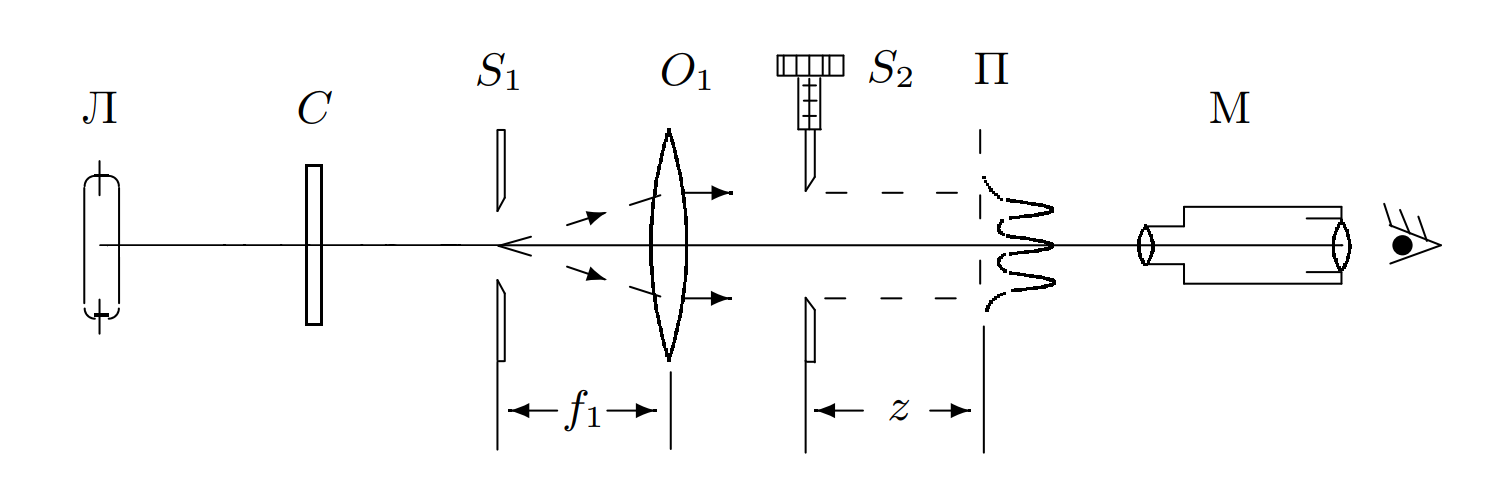
\includegraphics[width=0.8\linewidth]{2.png}
	\caption{Установка для наблюдения дифракции Френеля на щели}
	\label{fig:дифракцияФренеляУстановка}
\end{figure}


\begin{figure}[h!]
	\centering
	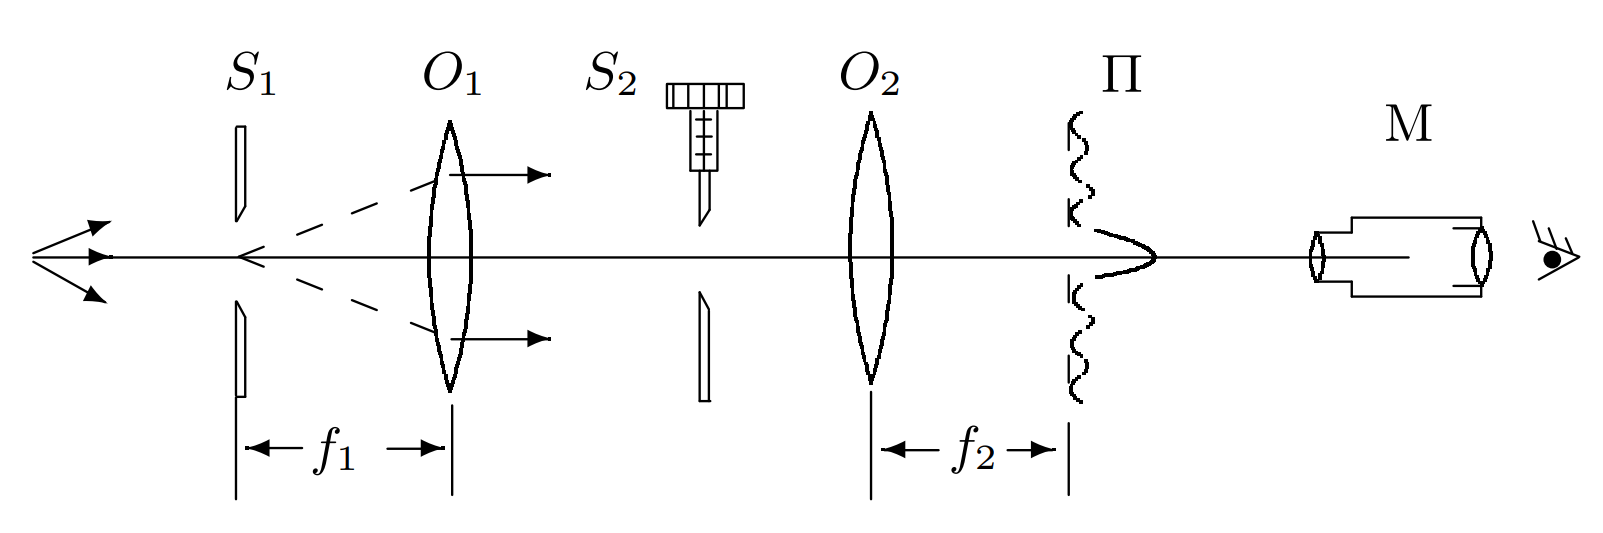
\includegraphics[width=0.8\linewidth]{3.png}
	\caption{Установка для наблюдения дифракции Фраунгофера на щели}
	\label{fig:Фраунгофер}
\end{figure}

\begin{figure}[h!]
	\centering
	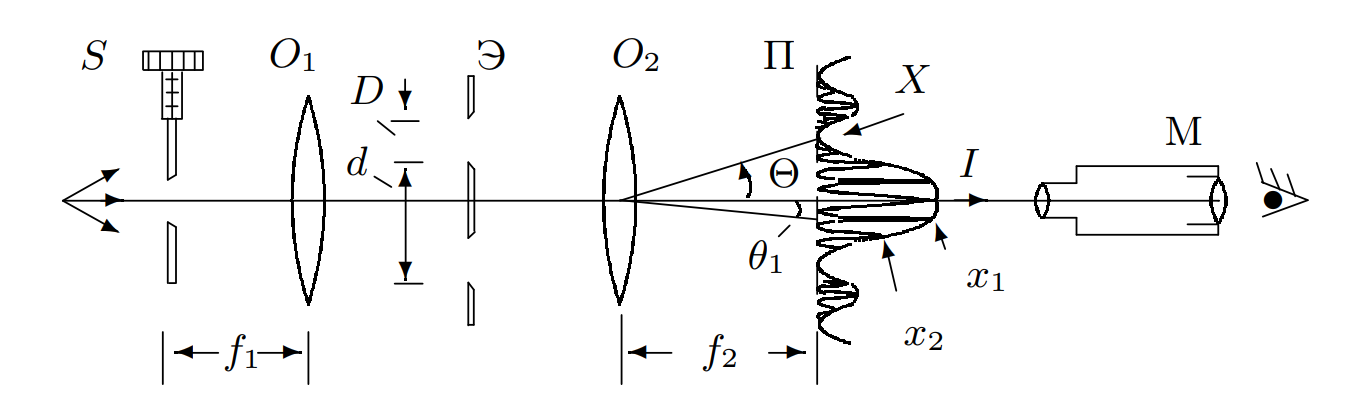
\includegraphics[width=0.8\linewidth]{4.png}
	\caption{Установка для наблюдения дифракции Фраунгофера на двух щелях}
	\label{fig:Фраунгофер2}
\end{figure}

\begin{figure}[h!]
	\centering
	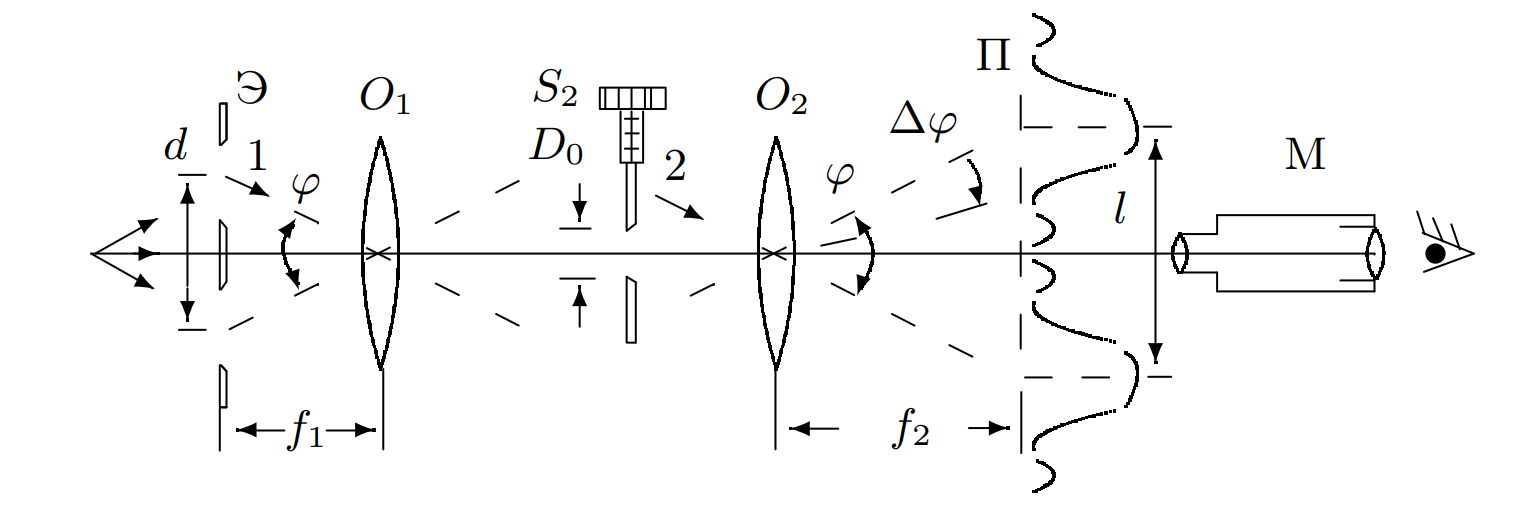
\includegraphics[width=0.8\linewidth]{9.png}
	\caption{Установка для исследования влияния дифракции на характеристики оптических приборов}
	\label{fig:послустановка}
\end{figure}


\section{Результаты измерений и обработка данных}

\subsection{Дифракция Френеля на щели и препятствии}

\paragraph{Настройка.}

Найдём нуль микрометра на щели:
\begin{equation*}\label{key}
	 b_0 = 0,81 \pm 0,001 \; мм.
\end{equation*}
Ширина щели по микрометрическому винту:
\begin{equation*}\label{key}
	b = 0.315 \pm 0.001 \; мм.
\end{equation*}
Методом последовательных приближений получим по возможности контрастную картину.

\paragraph{Измерения.}

\begin{figure}[h!]
	\centering
	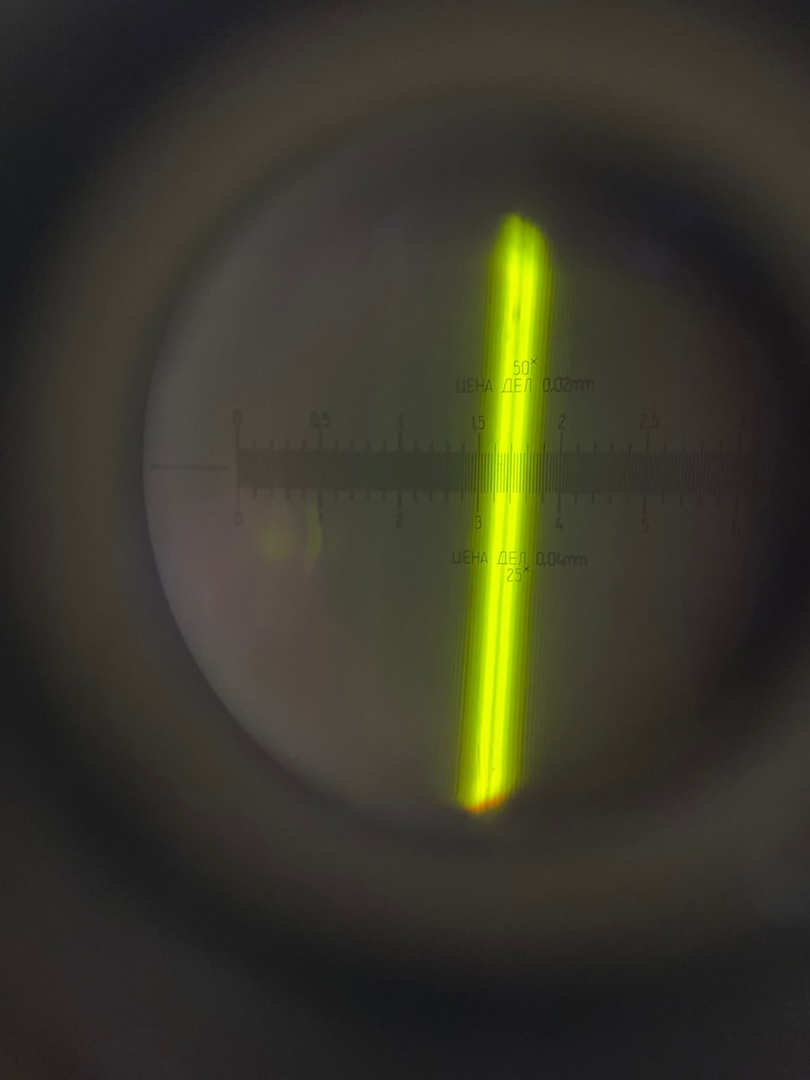
\includegraphics[width=0.5\linewidth]{frenel.jpg}
	\caption{Наблюдение тёмной полосы на фоне щели}
	\label{fig:1полоса}
\end{figure}

Найдём начальное положение микроскопа (без дифракции):
\begin{equation*}\label{key}
	L_0 = 624 \pm 2\; мм.
\end{equation*}
Получим зависимость количества полос от расстояния в табл. \ref{tab:Френель}. По формуле \eqref{eq:шустерзоны} рассчитаем величину $2\xi_n$, где $n = m + 1$. 
\begin{table}[h!]
	\centering
	\begin{tabular}{|c|c|c|c|c|}
    \hline
    $m$ & $L$, см & $z$, см & $n$ & $\xi_n$, мм \\ \hline
    0 & 62,4  & 0,0   & 1 & 0,00       \\ \hline
    1 & 63,0  & 0,6   & 2 & 0,08       \\ \hline
    2 & 63,9  & 1,5   & 3 & 0,16       \\ \hline
    3 & 64,2  & 1,8   & 4 & 0,20       \\ \hline
    4 & 64,4  & 2,0   & 5 & 0,23       \\ \hline
    5 & 64,6  & 2,2   & 6 & 0,27       \\ \hline
    6 & 64,7  & 2,3   & 7 & 0,30       \\ \hline
    \end{tabular}
    \caption{Зависимость количества тёмных полос от расстояния}
	\label{tab:Френель}
\end{table}

В этой таблице возьмём инструментальную погрешность $ \Delta = 2 \; мм $.
При помощи микрометрического винта на микроскопе и шкалы на окуляре найдём ширину щели:
\begin{equation*}\label{key}
	b^{микроскоп} = 0.30\pm 0.02 \; мм.
\end{equation*}
По микрометру на щели,
\begin{equation*}\label{key}
	b^{микрометр} = 0.315\pm 0.01 \; мм.
\end{equation*}
Значит, люфтом можно пренебречь.

\paragraph{Качественные наблюдения.}

При уменьшении щели уменьшается количество дифракционных полос. Это согласуется с теорией и обусловлено возрастанием волнового параметра \eqref{eq:волновойПараметр}.

Для дифракции Френеля на препятствии в виде тонкой вертикальной нити при удалении микроскопа -- чётное число тёмных полос.

\begin{figure}[h]
		\begin{minipage}[h]{0.4\linewidth}
			\center{\includegraphics[width=0.9\linewidth]{yarn1.jpg}}
		\end{minipage}
		\hfill
		\begin{minipage}[h]{0.4\linewidth}
			\center{\includegraphics[width=0.9\linewidth]{yarn2.jpg}}
		\end{minipage}
		\hfill
		\caption{Наблюдение тёмных полос на фоне нити}
		\label{fig:yarn}
	\end{figure}

\paragraph{Обработка данных.}

Сравним размер зон Шустера с шириной щели $ S_2 $. Построим график на рис. \ref{fig:ФренельГрафик}.
\begin{figure}[h!]
	\centering
	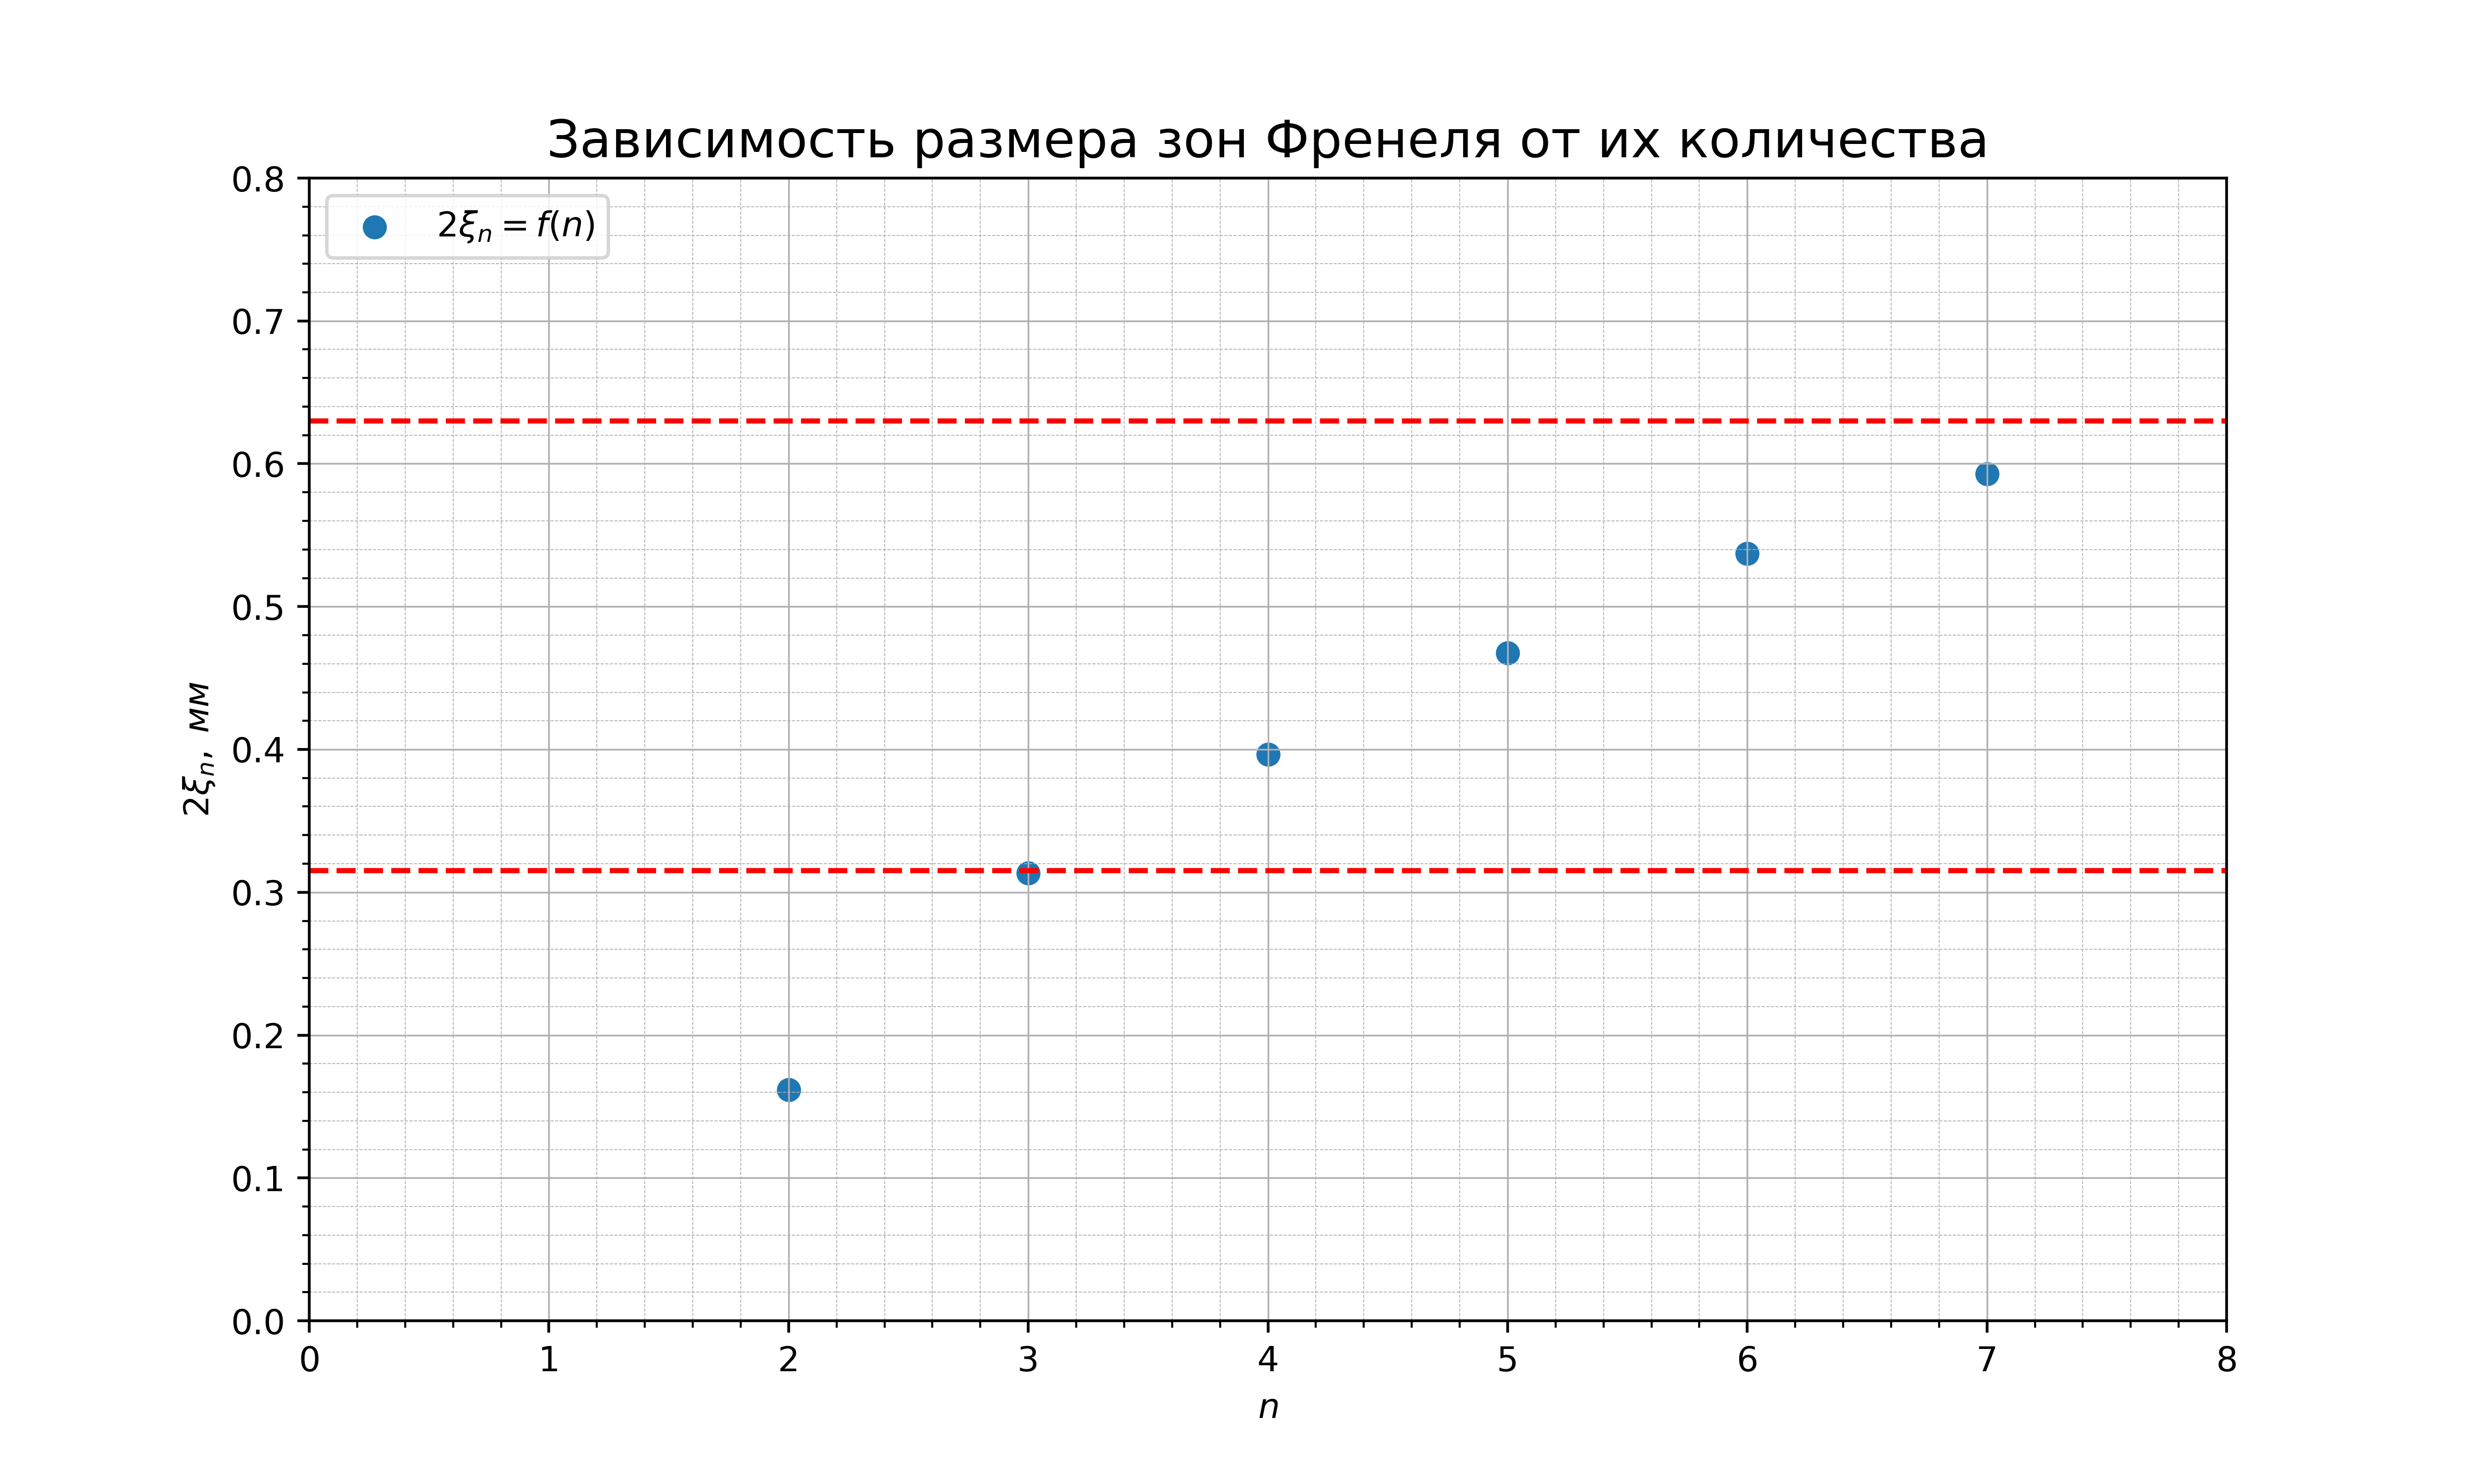
\includegraphics[scale=0.7]{4.3.1_1.png}
	\caption{Ширина зон Шустера}
	\label{fig:ФренельГрафик}
\end{figure}

\newpage

\subsection{Дифракция Фраунгофера на щели}

\paragraph{Настройка.}

Фокус линзы-объектива $ O_2 $ равен $ 12.8\pm 0.1\; см $.
Получена дифракционная картина Фраунгофера на всё поле зрения микроскопа. 

\paragraph{Измерения.}

\begin{figure}[h!]
	\centering
	\includegraphics[width=0.5\linewidth]{difr.jpg}
	\caption{Наблюдение дифракции Фраунгофера на щели}
	\label{fig:fraungDif}
\end{figure}

Снимем значения координат нескольких дифракционных минимумов в табл.~\ref{tab:Фраунгофер}.
\begin{table}[h]
	\centering
	\begin{tabular}{|c|c|c|}
    \hline
    $m$  & $X_m$, дел & $X_m$, мм  \\ \hline
    1  & 2,21  & 0,004  \\ \hline
    2  & 2,41  & 0,008  \\ \hline
    3  & 2,62  & 0,012  \\ \hline
    4  & 2,83  & 0,017  \\ \hline
    5  & 3,09  & 0,022  \\ \hline
    -1 & 1,75  & -0,005 \\ \hline
    -2 & 1,54  & -0,009 \\ \hline
    -3 & 1,34  & -0,013 \\ \hline
    -4 & 1,13  & -0,017 \\ \hline
    -5 & 0,93  & -0,021 \\ \hline
    \end{tabular}
	\label{tab:Фраунгофер}
	\caption{$ X_m (m) $ для опыта Фраунгофера }
\end{table}

Погрешность $ X_m $ в этой таблице считаем равной цене деления $ 0.02\; мм $. Ширина щели в этом опыте:
\begin{equation*}\label{key}
	b = 0.350 \pm 0.001 \; мм.
\end{equation*}

\paragraph{Качественные наблюдения.}

При смещении $ S_1 $ не происходит сдвига дифракционной картины. Это связано с тем, что картина находится в фокальной плоскости линзы $ O_2 $, куда приходят почти параллельные лучи.

При уменьшении ширины щели картина растягивается, что согласуется с формулой~\eqref{eq:ФраунгоферМинимумы}.

\paragraph{Обработка данных.}

Построим график зависимости координаты $ X_m (m) $ на рис.\ref{fig:Дифрграфик}.
\begin{figure}[h!]
	\centering
	\includegraphics[scale=0.7]{4.3.1_2.png}
	\caption{Зависимость координаты минимума интенсивности от его номера}
	\label{fig:Дифрграфик}
\end{figure}

\newpage

Получаем результат
\begin{equation*}\label{key}
	\Delta X_m \approx (43\pm 1) \cdot 10^{-4} \; мм
\end{equation*}

По формуле \eqref{eq:ФраунгоферМинимумы} определяем $$b = \frac{\lambda}{\Delta X_m}f_2 = 0,30 \pm 0,01~мм$$.

\subsection{Дифракция Фраунгофера на двух щелях}

\paragraph{Настройка и измерения.}

Получим по возможности чёткую дифракционную картину. Ширина центрального максимума при $ b=0.060\pm 0.001\; мм $ равна
\begin{equation*}\label{key}
	X = 0.01\pm 0.001 \;мм,
\end{equation*}
и он включает в себя $ n = 8 $ светлых промежутков.
Первое исчезновение интерференционных полос при
\begin{equation*}\label{key}
	b_0 = 0.10 \pm 0.01 \;мм.
\end{equation*}

\paragraph{Обработка результатов.}

\begin{figure}[h!]
	\centering
	\includegraphics[width=0.5\linewidth]{2difr.jpg}
	\caption{Наблюдение дифракции Фраунгофера на двух щелях}
	\label{fig:fraung2Dif}
\end{figure}

Расстояние между минимумами равно:
\begin{equation*}\label{key}
	\delta x \approx \frac{X}{n} = 0.119\pm 0.003 \; мм.
\end{equation*}
Из формулы \eqref{eq:ИнтерфПолосыФраунгоф2}:
\begin{equation*}\label{key}
	d = \frac{\lambda f_2}{\delta x} = 0.59\pm 0.01 \; мм.
\end{equation*}
Это значение отличается от замеренного: фактическое расстояние между щелями около $ 0.77\pm 0.01\; мм $. Расхождение может быть связано с неодинаковым расстоянием между щелями.

\subsection{Влияние дифракции на разрешающую способность оптического инструмента}

\paragraph{Настройка и измерения.}
Найдём минимальную ширину щели $ S_2 $, при которой изображения двух щелей ещё различимы:
\begin{equation*}\label{key}
	b_0 = 0.13\pm 0.01 \; мм.
\end{equation*}
Геометрические размеры щелей:
\begin{equation*}\label{key}
	d_1 = 0.16 \pm 0.01 \; мм,
\end{equation*}
\begin{equation*}\label{key}
	d_2 = 0.23 \pm 0.01 \; мм,
\end{equation*}
\begin{equation*}\label{key}
	d = 0.77 \pm 0.01 \; мм,
\end{equation*}
где $ d $ --- расстояние между щелями.

\paragraph{Обработка данных.}

Оценим выполнение критерия Рэлея. Из \eqref{eq:рэлей},
\begin{equation}\label{eq:last}
	b_0 = \frac{\lambda f_1}{d} = 0.09\pm 0.01\; мм.
\end{equation}
Значительное расхождение, вероятно, связано с субъективностью оценки <<щели всё ещё различимы>>. 

\section{Вывод}

В данной работе изучались явления дифракции Френеля и Фраунгофера. Провели сравнение установок, применяемых в этих опытах. Выявили различия этих двух явлений. Провели ряд сравнений значений, полученных экспериментально, с расчётными. В нескольких случаях их несовпадения могут быть вызваны субъективностью визуальной оценки.

Исследовали влияние дифракции Фраунгофера на оптические приборы. Установили связь между уменьшением диафрагмы прибора и ухудшением разрешения, связанным с дифракцией.

С помощью качественных наблюдений установили ряд различий между исследуемыми явлениями и их особенности.

\end{document}
